% Author: Mark G.

\subsubsection{Description/additional circuitry}
% Describe how your electronic hardware brake plausibility system works (this is in addition to your ECU controlled brake plausibility software), provide tables with main operation parameters, and describe additional circuitry used to check or for an implausibility. Describe how the system reacts if an implausibility or error is detected.

\Acrfull{bspd} is represented by a \gls{pcb} with an on-board current transducer. It’s function is to monitor
power drawn from \gls{acp} and brake pedal pressure, and open \gls{sdc} in case both signals are above
allowed threshold for more than 0.5 seconds. Also, the event of disconnection of \gls{sdc} is latched,
thus it gets to reset only in case of the main power reset.


\begin{table}[H]
	\centering
	\caption{BSPD data}
	\begin{tabu}{|X|X|}
		\hline
		Brake sensor used: & Piezoresistive Pressure Transmitter PA-21Y / 100bar / 81691.1 \\
		\hline
		Brake sensor physical response value: & Voltage, 4.5 \vdc \\
		\hline
		Tractive system power sensor type & Current Transducer LEM HTFS 200-P \\
		\hline
		Tractive system sensor physical response value: & Voltage of 85 mV \\
		\hline
		Tractive System power sensor current threshold (5 kW/Nominal \gls{ts} voltage): & 14 A \\
		\hline
		Supply voltages: & 5 V \\
		\hline
		Maximum supply currents: & 22 mA \\
		\hline
		Operating temperature: & -40 \degC to 105 \degC \\
		\hline
		Output used to control \glspl{air}: & Open a MOSFET in \gls{sdc} \\
		\hline
	\end{tabu}%
	\label{tab:bspd}%
\end{table}%

Complete datasheet: \ref{app:bspd_lem_datasheet}

\iffalse
\begin{figure}[H]
	\centering
	\includegraphics[width=\textwidth]{./img/bspd-position.jpg}
	\caption{\Gls{bspd} flowchart.}
	\label{fig:BSPD-flowchart}
\end{figure}\fi

\subsubsection{Schematic}
%Describe the wiring, show schematics including the circuit board, show data regarding the cables and connectors used
The \gls{bspd} \gls{pcb} is mounted on a \gls{hv} wire in such manner, that the \gls{hv} wire goes through the
current transducer. Current transducer provides analog voltage output of a value proportional to
actual current (resp. power) drawn from \gls{acp}. This voltage is amplified and is converted to two-state
logic levels voltage with the use of comparators. The value of “High” current signal logic level
is set to be at 5 kW of power drawn from \gls{acp} (14 A).

Brake state is measured in \gls{ecup}, converted with help of a comparator to two-state logic levels
voltage and is sent directly to \gls{bspd} via wiring.

Both logic signals are connected to NAND inputs. When both inputs are at “High” level, a
capacitor $C_1$ starts to charge through resistance $R_{16}$. When voltage on $C_1$ is higher than 2.5V, a
comparator $U_{1B}$ sends signal to open \gls{sdc}.

\begin{figure}[H]
	\centering
	\includegraphics[width=\textwidth]{./img/bspd-schematic.pdf}
	\caption{\gls{bspd} schematic sheet}
	\label{fig:BSPD-schematic}
\end{figure}

\subsubsection{Connection with shutdown circuit}
The connection to \gls{sdc} is provided by an NPN transistor $Q_2$ and a P-Channel MOSFET $Q_1$, that
are connected to act as a “normally-closed” switch in \gls{sdc} loop. Thus in case of a trip event $Q_1$
stops conducting current between Drain and Source. See \ref{fig:BSPD-schematic}.

This state is latched by a latch-circuit, that consists of two NAND gates.

\iffalse
\begin{figure}[H]
	\centering
	\includegraphics[width=\textwidth]{./img/bspd-position.jpg}
	\caption{\gls{bspd} connection with \gls{sdc}.}
	\label{fig:BSPD-conn}
\end{figure}\fi

\subsubsection{Position in car/mechanical fastening/mechanical connection}
%Provide CAD-renderings showing all relevant parts and discuss the mechanical connection of the sensors to the pedal assembly. Mark the parts in the rendering, if necessary.

\gls{bspd} is placed in Service Box, which connects high voltage harnesses from accumulator pack to motor controllers. The board containing \gls{bspd} circuit and current transducer is mounted to a wire.
\begin{figure}[H]
	\centering
	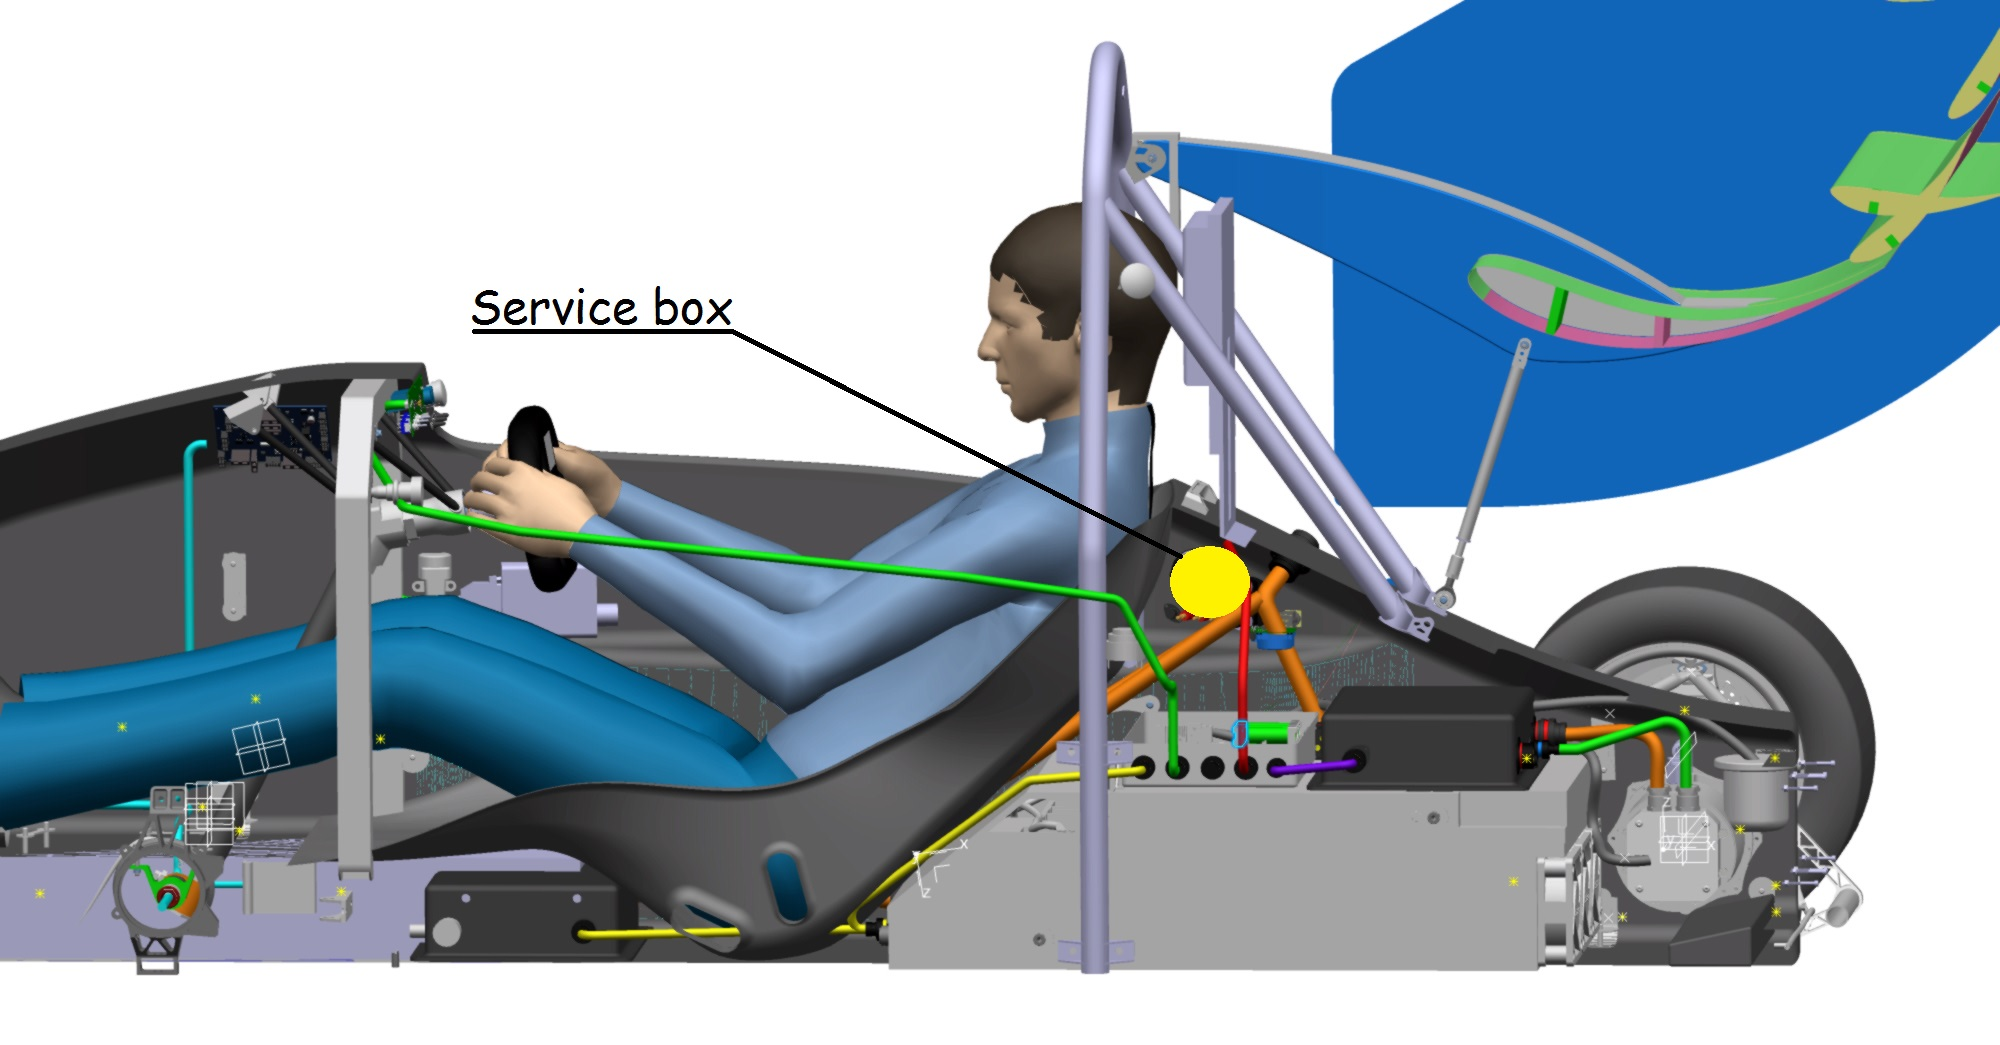
\includegraphics[width=\textwidth]{./img/ServiceBox-position.jpg}
	\caption{\gls{bspd} position}
	\label{fig:BSPD-position}
\end{figure}
